\documentclass{article}
\usepackage{amsmath}
\usepackage{graphicx}
\usepackage{listings}
\usepackage{dirtytalk}
\usepackage{hyperref}

\hypersetup{
    colorlinks=true,
    linkcolor=magenta,    
    urlcolor=magenta
}

% Polish language support
\usepackage[utf8]{inputenc}   % Encoding of the input file (UTF-8)
\usepackage[T1]{fontenc}       % Output font encoding
\usepackage[polish]{babel}     % Polish language support

\title{Opis modelu matematycznego - dopasowanie modelu logistycznego z członem wielomianowym do danych COVID-19}
\author{}
\date{}

\begin{document}

\author{Artur Bieniek}
\maketitle

\say{Jest 01:37, zabieram się do pisania swojej pierwszej w życiu notatki w \TeX-u, to będzie ciekawa noc...} - powiedział na pewno ktoś kiedyś

\section{Wstęp}
Celem niniejszej notatki jest przedstawienie modelu matematycznego, który służy do dopasowania danych dotyczących liczby aktywnych przypadków w pandemii. Model ten łączy funkcję logistyczną z dodatkowym składnikiem wielomianowym, aby umożliwić uchwycenie zarówno charakterystyki szybkiego wzrostu w początkowych etapach pandemii, jak i późniejszego wygaszania wzrostu.

\section{Model Matematyczny}

Model matematyczny, który wykorzystuję, jest rozszerzoną wersją klasycznego modelu logistycznego. W skład modelu wchodzi człon logistyczny oraz jeden dodatkowy człon wielomianowy, który wprowadza większą elastyczność w modelowaniu krzywej.

Model ma postać:
\[
f(x) = \frac{L}{1 + e^{-k(x - x_0)}} + (ax^4+bx^3)
\]
gdzie:
\begin{itemize}
    \item $f(x)$ - liczba aktywnych przypadków w dniu $x$ (liczba dni od pierwszego przypadku),
    \item $L$ - maksymalna wartość, do której zbliża się liczba przypadków (asymptota),
    \item $k$ - współczynnik szybkości wzrostu przypadków,
    \item $x_0$ - punkt infleksji, który określa dzień, w którym tempo wzrostu zaczyna zwalniać,
    \item $(ax^4+bx^3)$ - wielomian stopnia 4 (człon $(cx^2+dx+e)$ nie okazał się grać dużej roli w kształcie funkcji),
    \item $x$ - liczba dni od pierwszego przypadku.
\end{itemize}

\subsection{Człon Logistyczny}
Człon logistyczny:
\[
\frac{L}{1 + e^{-k(x - x_0)}}
\]
jest klasycznym modelem wzrostu, który początkowo wykazuje szybki przyrost, a następnie wygasza wzrost w miarę zbliżania się do wartości asymptotycznej $L$. Funkcja ta dobrze opisuje wiele procesów biologicznych i epidemiologicznych, w tym rozprzestrzenianie się chorób zakaźnych, które w początkowej fazie mają gwałtowny wzrost, a później spowalniają w wyniku różnych czynników, takich jak wyczerpywanie się zasobów lub wprowadzenie środków zapobiegawczych.

\subsection{Człon wielomianowy}
Człon wielomianowy:
\[
(ax^4+bx^3)
\]
wprowadza dodatkową elastyczność do modelu, pozwalając na uchwycenie nieliniowych zmian w przebiegu epidemii. Współczynniki niższych potęg można zupełnie pominąć bez utraty dopasowania. Zwiększenie stopnia wielomianu powyżej 6 prowadzi do wystąpienia poważnych problemów numerycznych, ponieważ docelowe wartości współczynników $a,b$ są bardzo małymi ułamkami.

\section{Dopasowanie Modelu do Danych}

Aby dopasować model do rzeczywistych danych, wykorzystuję metodę aproksymacji średniokwadratowej, której celem jest minimalizacja sumy kwadratów różnic między wartościami rzeczywistymi a wartościami przewidywanymi przez model. Dopasowanie to wykonuję przy pomocy funkcji \texttt{curve\_fit} z biblioteki \texttt{scipy.optimize}, która pozwala na optymalizację parametrów modelu.

Funkcja \texttt{curve\_fit} wymaga podania następujących argumentów:
\begin{itemize}
    \item Funkcja modelu, która opisuje zależność między zmiennymi niezależnymi a zależnymi,
    \item Zmienna niezależna ($x$) - w tym przypadku liczba dni od pierwszego przypadku,
    \item Zmienna zależna ($y$) - liczba aktywnych przypadków,
    \item Początkowe wartości parametrów (szacowane na podstawie danych lub wiedzy na temat modelu)
    \item $maxfev$ - liczbę maksymalnych iteracji, domyślnie jest ona zbyt mała
\end{itemize}

Na podstawie tych danych, funkcja \texttt{curve\_fit} zwróci optymalne wartości parametrów $L$, $k$, $x_0$, $a$ i $b$, które najlepiej pasują do rzeczywistego przebiegu danych.

\section{Interpretacja Parametrów}
Po dopasowaniu modelu do danych, otrzymujemy optymalne wartości parametrów, które pozwalają na interpretację zachowania epidemii:
\begin{itemize}
    \item $L$ wskazuje maksymalną liczbę przypadków, do której może dojść w populacji.
    \item $k$ określa szybkość wzrostu liczby przypadków w początkowej fazie epidemii.
    \item $x_0$ informuje o dniu, w którym tempo wzrostu przypadków zaczyna zwalniać.
    \item $a$ i $b$ umożliwiają dopasowanie krzywej do nieliniowych trendów, które mogą występować w danych.
\end{itemize}

\section{Dane}
Zgodnie z zasadą \say{śmieci na wejściu - śmieci na wyjściu} szukałem przez chwilę w internecie dobrego, zaufanego źródła danych w strawnym formacie, jednak ostatecznie zdecydowałem się wykorzystać zarekomendowany zestaw danych z
\href{https://docs.google.com/spreadsheets/d/1ierEhD6gcq51HAm433knjnVwey4ZE5DCnu1bW7PRG3E/edit?gid=1400401584#gid=1400401584}
{tego linku}. Był on o tyle wygodny, że wystarczyło zmienić nazwę kolumny z sumaryczną liczbą przypadków zachorowań od początku epidemii i używać wartości z kolejnych wierszy jako wskazań dla kolejnych dni.

\pagebreak
\section{Kod w Pythonie}
\lstinputlisting[language=Python]{9.py}

\section{Osiągnięte parametry}
\begin{itemize}
    \item L = 6454970.70
    \item k = 0.0161
    \item x0 = 336.46
    \item a = 0.000103
    \item b = -0.077099
\end{itemize}

\section{Efekt}
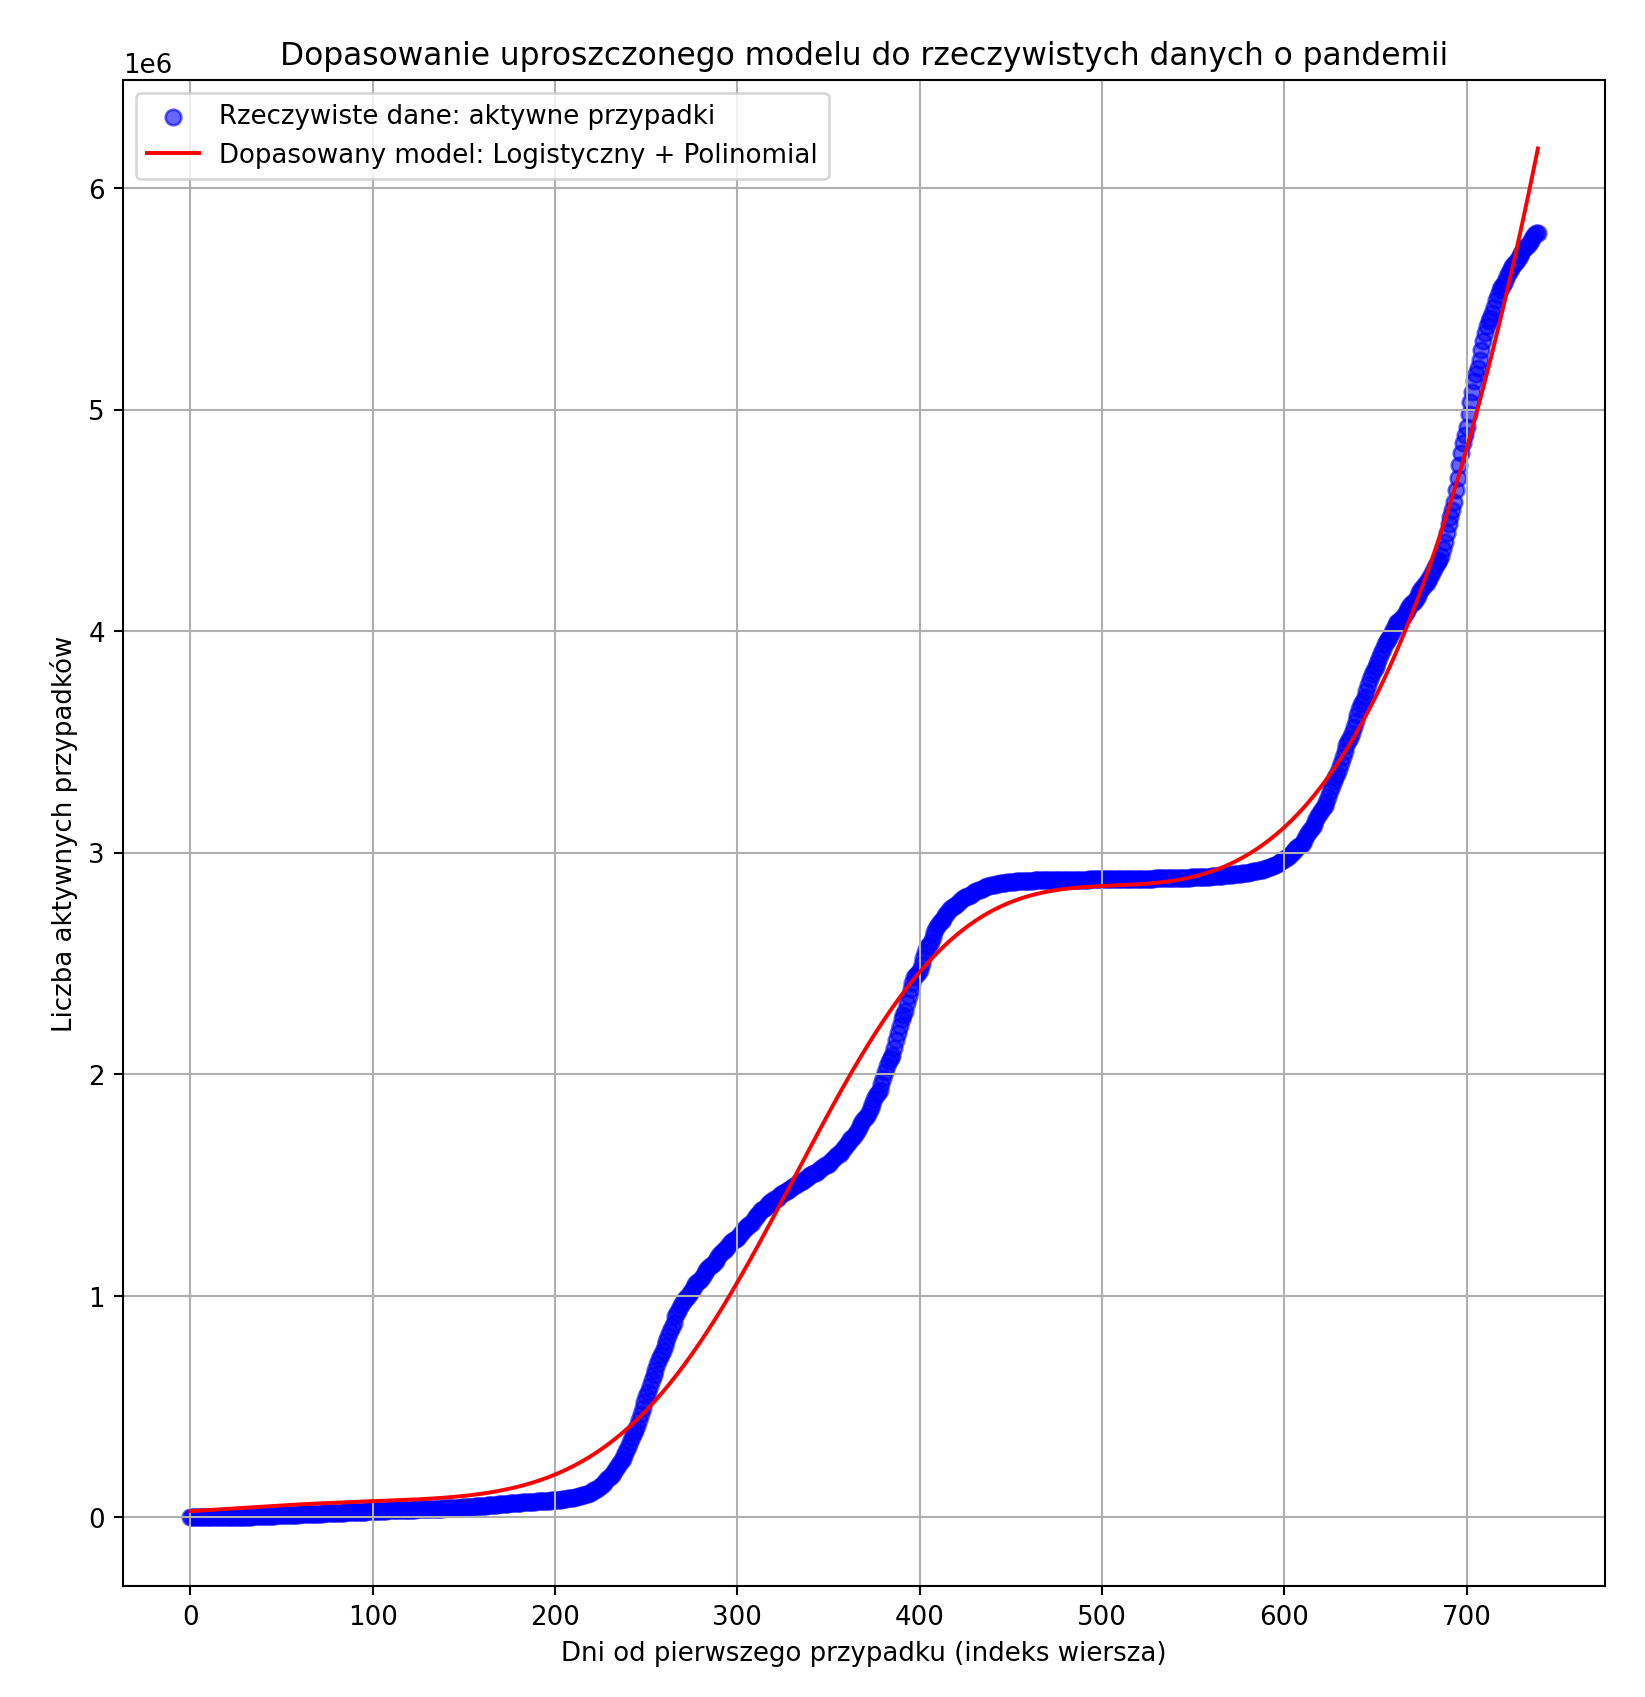
\includegraphics[width=\textwidth]{9.png}

\section{Podsumowanie}
Trzeba przyznać zgodnie z prawdą, że opracowany przeze mnie model jest prawdopodobnie bezużyteczny. Niemniej jednak, tworząc go:
\begin{itemize}
    \item Dowiedziałem się, że istnieje coś takiego jak model logistyczny
    \item Nauczyłem się świadomie korzystać z potężnego narzędzia do dopasowywania modeli (scipy)
    \item Napisałem pierwszy raz w życiu cokolwiek w \LaTeX, przy okazji całkiem nieźle się go nauczyłem
    
\end{itemize}
Także zdecydowanie nie można odmówić temu zadaniu wartości edukacyjnej.
\end{document}
